\chapter{Enabling Temporal Neural Networks via Geometric Tensor Representations} \label{chap:ott} 

The above statistical methods work well with
multivariate types of data and scale reasonably well with many features.
However,
even though we have a linear time scanning procedure,
if the number of features reaches thousands or more,
computational feasibility can still be an issue.
Particularly when we are not dealing with
imaging summaries,
using the explicit pixel or voxel-level
data is still intractable.
In these cases,
deep learning methods have
proven to be extremely effective
in modeling high-dimensional data.
Compbined with methods
for temporal modeling,
some success has been seen
in modeling imaging trajectories.
However, a separate problem
emerges: the \textbf{model size}
grows very large, linearly 
in the length of the temporal sequence of interest.
In this chapter, we examine
a novel tensor decomposition
that reduces this model size,
enabling the modeling of high-dimensional
temporal medical imaging data
with reasonable computational resources.

% intro to graphical models
Multivariate data analysis exploiting the conditional independence structure between features or covariates using 
undirected graphical models is now standard within any data analysis toolbox. 
When the data are multivariate Gaussian, the zeros in the inverse covariance (precision) matrix give conditional independences 
among the variables \cite{lauritzen1996graphical}. Further, if the precision matrix is sparse, we can  
derive dependencies between features when the data are high-dimensional and/or the number of measurements are small. 
The estimation of a graphical model
has been extensively studied
%in statistics and machine learning,
and a rich literature is available describing 
its statistical and algorithmic properties \cite{koller2009probabilistic,jordan1998learning}. 
%Particularly for higher-dimensional settings where the dimension $p$ is allowed to grow, \textit{sparse} estimation of the precision matrix has been well-studied. 
For instance, the so-called \textit{graphical lasso} formulation uses an $\ell_1$-norm penalty on the 
precision matrix and is widely used, and consistency properties 
in the large $p$ regime \cite{cai2011constrained,friedman2008sparse,yuan2010high} are now well understood. 
These formulations have also been extended to various transformations of Gaussian distributions (e.g., non-paranormal)
%, where the 
using rank statistics \cite{liu2009nonparanormal,xue2012regularized,liu2012high}.
%are a consistent estimator of 
%the precision matrix nonzero pattern 

{\em Coupled and Temporal Graphical Models.} 
%In various situations,
Often, data come from two (or more) disparate sources or multiple timepoints.
%, where we seek to estimate 
%a model for each source {\em independently}.
%When the sources share the same variables as well as the
%nd a non-trivial portion 
%of the
%dependency structure, we may decide to pool the data together and estimate a single model in an effort to boost statistical power. However, 
%such an approach invariably masks the heterogeneity in the data-set sources \cite{friston2011functional}. While we want 
%to preserve the common structure, ideally, we also wish to allow for differences among the 
%sources. Consequently, w
Within the last few years, a few proposals have 
described strategies for linking the sparsity patterns of multiple graphical models, e.g., using a fused lasso 
penalty \cite{danaher2014joint} \cite{yang2015fused}. Observe that 
%these ideas assume that the two (or more) models share a similar structure; 
if the data sources correspond to {\em longitudinal} acquisitions, we should expect 
the `structure' to gradually evolve.
%, which is discouraged in direct applications of the above idea. 
%in the case where the model is changing such a construction would not allow for identification of the evolving graph structure. 
Several authors have offered generalizations to address this problem: \cite{zhou2010time} removes the assumption
that each graph is independent and structurally `close'.
Instead, \cite{zhou2010time} can be thought of as a growth model \cite{mcardle2000introduction} defined on these structures: they show how non-identically distributed graphs can be learned over time. 
Recently, the nonparametric procedure in \cite{qiu2015joint} extends these ideas
%via means
to handle multiple sources, each with multiple samples.

The ideas in the literature so far to ``couple'' multiple graphical model estimation modules are mostly nonparametric. 
While such a formulation offers benefits, in many estimation problems, 
parametric models may 
%require fewer samples (better convergence rates) and possibly, 
be more convenient for downstream statistical analysis,
particularly for hypothesis testing \cite{hardle1993comparing,geer2000empirical,roehrig1988conditions}.
Given that the topic of \textit{coupled} graphical models, by itself, is fairly recent, algorithms for {\em parametric estimation} of 
temporal or coupled Gaussian graphical models have not yet been heavily studied. 
%Part of the reason is the difficulty of 
This will involve parameterizing {\em trends} in the highly structured nature of the `response' variable ($\SPD$ matrices). 
%In contrast, w
We find that parametric formulations for manifold-valued data {\em have} been proposed recently \cite{hjkimcvpr2014,cornea2016regression}. %, albeit only in the 
%context of regression models and dictionary learning \cite{xie2013nonlinear}. 
%This result is relevant --- b
Because $\SPD$ matrices form a Riemannian manifold, algorithms
that estimate a parametric model respecting the underlying Riemannian metric are more suitable in many applications as opposed to assuming a Euclidean metric 
on positively or negatively curved spaces \cite{xie2010statistical, fletcher2007riemannian, jayasumanakernel}. We will make a few simple modifications 
(for efficiency purposes) to such algorithms and make use of the estimated parameters for follow-up analysis.

%Unfortunately, their deployment for the $\SPD$ may not always be trivial.

{\em Finding Group-wise Differences.} Assuming that we have a black-box procedure to estimate a parametric model on the $\SPD$ manifold available, 
in many tasks, such an estimation is merely a segue to other analyses designed to answer scientifically meaningful questions. 
For example, we are often interested in asking whether the temporally coupled model estimated using the procedure above differs 
in meaningful ways {\em across} groups induced by a stratification or dichotomous variable (e.g., gender or disease). For instance, is the `slope' in structured response space statistically different 
across education level or body mass index? 
%in if this model differs significantly across two groups.
While the body of work for graphical model estimation is mature, the literature describing hypothesis tests in this
regime \cite{diffnet,belilovsky2015hypothesis}
is sparse at best.
%When considering a single graphical model for each group, \cite{diffnet} propose a framework for two sample testing to discover differences in biological network structures.
%However, to the best of our knowledge no literature exists describing a testing framework for temporal graphical models.
%In this paper we propose a method for evaluating this group difference temporally.
Given that such questions are simpler to answer with alternative schemes (with assumptions on the distributional properties of the data), e.g., structural equation modeling, 
latent growth models and so on \cite{ullman2003structural, mcardle2000introduction}, it seems that 
the unavailability of such tools is limiting the adoption of such ideas in a broader 
cross-section of science. We will seek to address this gap. 

{\em Needles in Temporal Haystacks.} If we temporarily set aside the potential value of a hypothesis test framework for temporal 
trajectories in graphical models, we see that
from an operational viewpoint, such procedures are most effective when a practitioner already has a precise scientific question in mind. In reality, however, 
many data analysis tools are deployed for exploratory analyses to inform an investigator as to which questions to ask. 
Being able to ``localize'' which parts of the model are different across groups over the entire time window can be very valuable. This ability actually 
benefits statistical power as well. Notice that when the stratified groups are not very different 
to begin with, e.g., healthy individuals with presence or absence of a genetic mutation, the
effect sizes are likely to be poor.
Here, while the trends identified on the {\em full} precision matrix may still be different (i.e., there may be a {\em real} signal 
associated with a grouping variable), 
they may not be strong enough to survive significance thresholds. Ideally, what we need here are analogs of the widely used ``scan statistics'' 
for our hypothesis testing formulations for temporal graphical models --- to identify which {\em parts of the signal} are promising. 
Then, even if only a small subset of 
features were different across groups over all time,
%(whereas the complement of this sub-graph were similar, i.e., not different)
we may be able to identify these differential effects efficiently. This benefits Type 2 error, 
provides a practical turnkey product for an experimental scientist, and makes up the key technical results of our work.

%motivation for our selection, cost etc.
%A second key issue we aim to address is that of feature selection. In many medical regimes, the true indicators and dependencies among measured features is unknown. In most analyses feature selection is done manually, generally by the researcher. Structural equation modeling (SEM) in particular is a popular tool which requires the user to choose the features as input for analysis. The first component of SEM requires the \textit{structural model} be specified, that the dependences we wish to determine significant are explicitly stated. Quantitative approaches for feature selection  (cite) have been looked at in machine learning. (elaborate)... In the case of image analysis, scan statistics have been used as a measure to detect regions of high correlation between images (cite what Ming cites). These scan statistics, however, require a selection of a subregion of the image or some strong heuristic to make the problem of searching over all possible window sizes tractable. Recently (ming paper) were able to polynomially bound the number of regions needed to detect highly correlated regions with high probability. Motivated by their work, we attempt to solve a parallel problem. In the case of feature selection among high-dimensional covariance matrices, we aim to identify a subset of features such that the evolution of the correlation matrix is significantly different among two groups.

% ULF GRENANDER
%\begin{mdframed}[hidealllines=true,backgroundcolor=blue!20]
Foundations of our work can be traced back to fundamental developments made by Ulf Grenander in a breadth of fields. Early work with Rosenblatt on the analysis of stochastic processes and time series first brought to light
the fundamental issues of linear modeling in Euclidean space, and demonstrated that in many cases it is necessary to develop methods that take explicit advantage of the inherent structure within data \citep{grenander1957statistical}.
Further pioneering work on the statistical analysis on Lie groups \citep{grenander2008probabilities} provides the basis of the Riemannian statistics mentioned above.
Modern hypothesis testing of these structured, manifold-valued data in image analysis is built upon the his joint work \citep{grenander1998computational}. Here, we marry modern developments in these areas, using recent strides in linear model fitting on manifolds and statistical testing of structured data to develop groupwise testing procedures for longitudinal covariances.
%\end{mdframed}
Concurrent to our work, \cite{su2014statistical,zhang2018rate} have developed similar methods of analyzing the statistical properties of trajectories on the $\SPD(n)$ manifold via the transported square-root vector field. While here we focus on a simple approach to enable localization, these developments can be incorporated into our construction.

Briefly, we provide \textbf{(i)} a simple and efficient parametric procedure for modeling temporally evolving graphical models, \textbf{(ii)} a 
hypothesis test for identifying differences between group-wise estimated models, and \textbf{(iii)} a scan
algorithm to identify {\em those subsets of the features which contribute to the group-wise differences}.
Together, these ideas offer a framework for identifying group-wise differences in temporally coupled graphical models.
%We next cover preliminary concepts, we define our model and present an algorithm, followed by experimental results on both simulated data and neuroimaging data 
%acquired from 
From the experimental perspective, we find scientifically plausible results on 
a unique longitudinally tracked cohort of middle-aged (and young elderly) persons at risk for Alzheimer's disease due to family history, 
but who are otherwise completely cognitively healthy.

The rest of the paper is organized as follows. In Section \ref{sec:mglm} we present an efficient manifold regression procedure for 
modeling covariance trajectories, which serves as a blackbox module in our hypothesis testing framework. 
In Section \ref{sec:hyp-test}, we define our main hypothesis test for group difference analysis over covariance trajectories. 
In Section \ref{sec:loc}, we present a set of technical results describing our localization procedure based on scan statistics, 
as well as derive suitable size corrections to compare across feature subsets. Sections \ref{sec:loceval}, \ref{sec:pipeval}, and \ref{sec:wrap} conclude with
empirical evaluations of our model on synthetic data, various types of demographics/behavior data collected longitudinally 
in the United States from publicly available resources, and finally, our 
analysis on a unique longitudinal dataset (followed since 2001) from a preclinical Alzheimer's disease study involving approximately 1500 individuals.

%\chapter{Ongoing Work: Large Scale Analysis of Multi-Site Preclinical Alzheimer's Disease} \label{chap:pac} 

With the above tools in hand, we aim to move towards applying and deploying both conditional independence schemes and efficient EMD-fairness methods to 
the analysis of a new preclinical cohort of individuals at risk for developing Alzheimer's disease.

\textbf{Data.} Here our data consists of patient information pooled across multiple sites. Demographic measures, neuropsychological test results, genetic indicators, and cerebrospinal fluid (CSF) biomarkers were all collected on individuals from three studies: the Adult Children Study (ACS), the Wisconsin Registry for Alzheimer's Prevention (WRAP), and the Biomarkers of Cognitive Decline Among Normal Individuals (BIOCARD). Data was preprocessed using standard pipelines, collated, and harmonized across sites. Table~\ref{tab:pacfeats} details the full list of measures.

\begin{table}
    \centering
    \begin{tabular}{l|l}
        \hline\hline
         A$\beta$42 & A$\beta$40 \\
         T-Tau & P-Tau \\
         A$\beta$42/A$\beta$40 & PTAU-A$\beta$42 \\
         Age & Gender \\
         Executive Function & General Cognitive Performance \\
         Episodic Memory & Time \\
         Education & APOE \\
         \hline\hline
    \end{tabular}
    \caption{Preclinical AD Measures used in conditional independence analysis.}
    \label{tab:pacfeats}
\end{table}

Imaging data is also available for a subset of the individuals included in the above set, and future work includes incorporation of these imaging modalities (MRI, DTI, and PET region of interest measures).

\textbf{Preliminary Methods and Results.} The results shown here demonstrate the potential value of applying conditional independence methods over standard correlation methods. The value of sparsity patterns derived from conditional independence testing appears to be clear, in that hyper-parameters need not be chosen in any way, compared to an $\alpha$-level for hypothesis testing via correlation coefficients, or a regularization level $\lambda$ for a typical graphical LASSO setting. Running the same analysis separately for each site, first observations indicate that there may exist dependencies and independencies unique to each study.

\begin{figure}
    \centering
    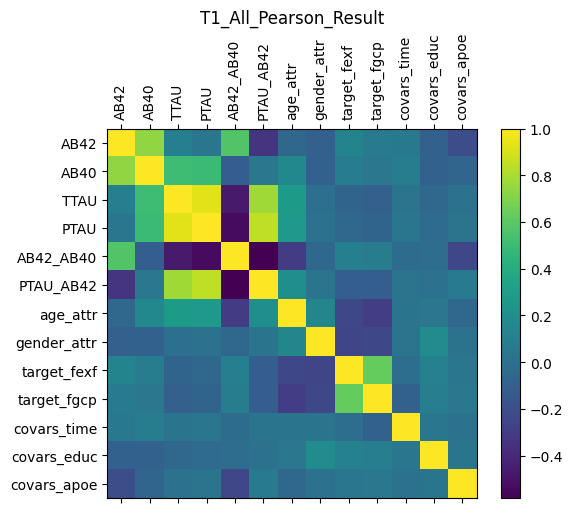
\includegraphics[width=0.24\textwidth]{diss/7_cond/figs/T1_All_Pearson_Result.png}
    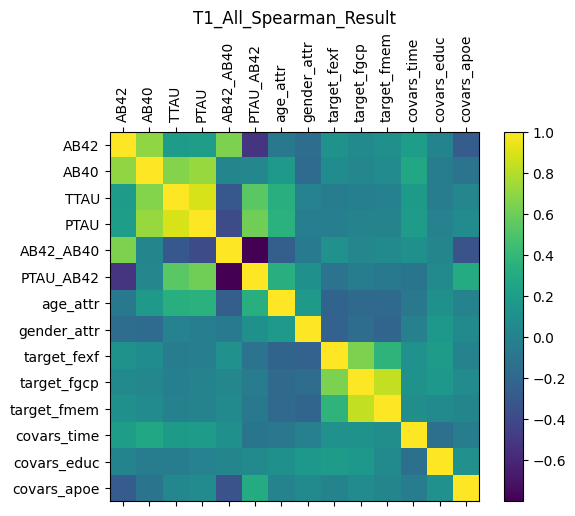
\includegraphics[width=0.24\textwidth]{diss/7_cond/figs/T1_All_Spearman_Result.png}
    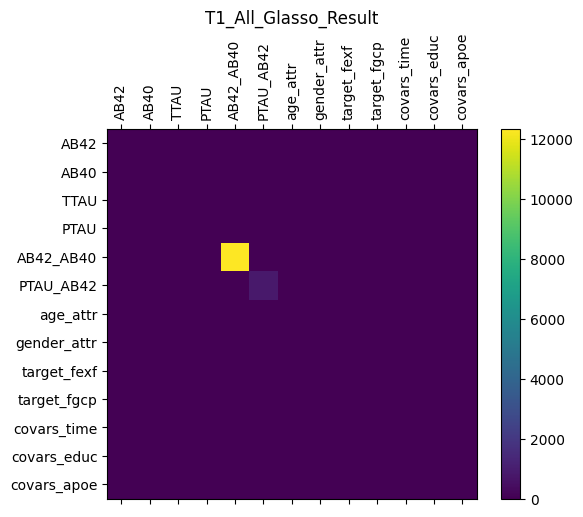
\includegraphics[width=0.24\textwidth]{diss/7_cond/figs/T1_All_Glasso_Result.png}
    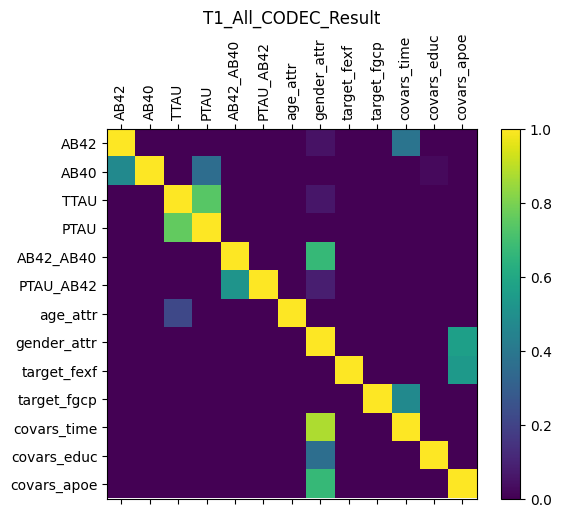
\includegraphics[width=0.24\textwidth]{diss/7_cond/figs/T1_All_CODEC_Result.png}
    
    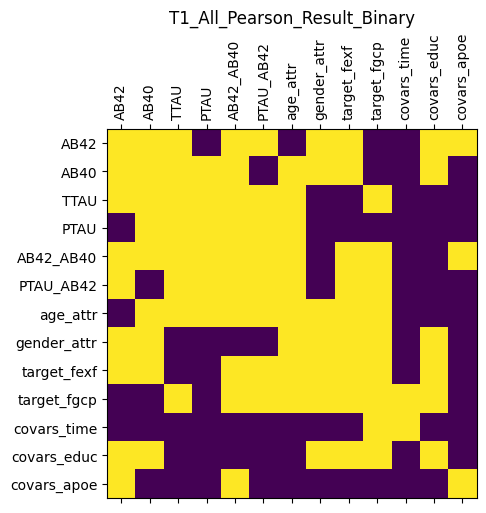
\includegraphics[width=0.24\textwidth]{diss/7_cond/figs/T1_All_Pearson_Result_Binary.png}
    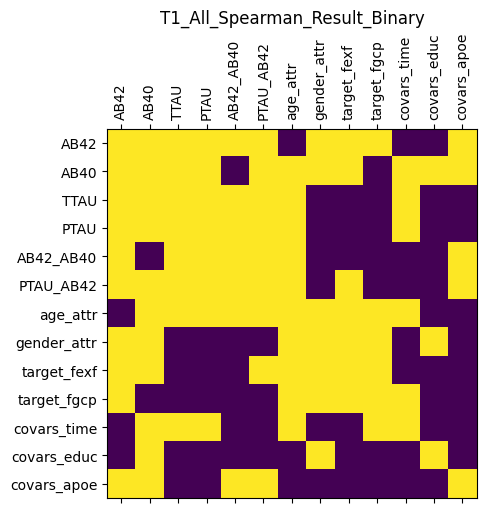
\includegraphics[width=0.24\textwidth]{diss/7_cond/figs/T1_All_Spearman_Result_Binary.png}
    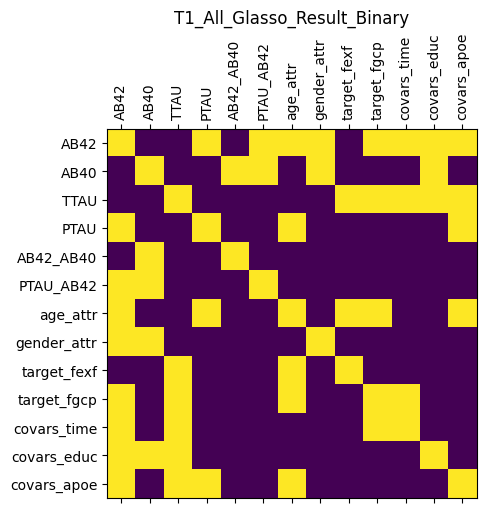
\includegraphics[width=0.24\textwidth]{diss/7_cond/figs/T1_All_Glasso_Result_Binary.png}
    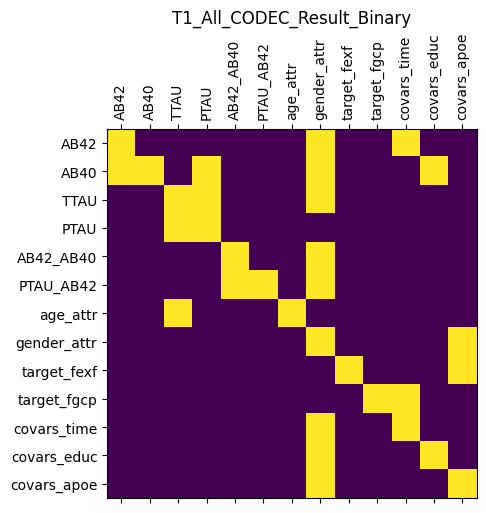
\includegraphics[width=0.24\textwidth]{diss/7_cond/figs/T1_All_CODEC_Result_Binary.png}
    
    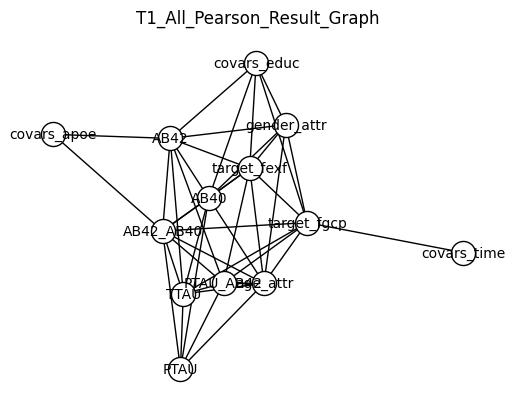
\includegraphics[width=0.24\textwidth]{diss/7_cond/figs/T1_All_Pearson_Result_Graph.png}
    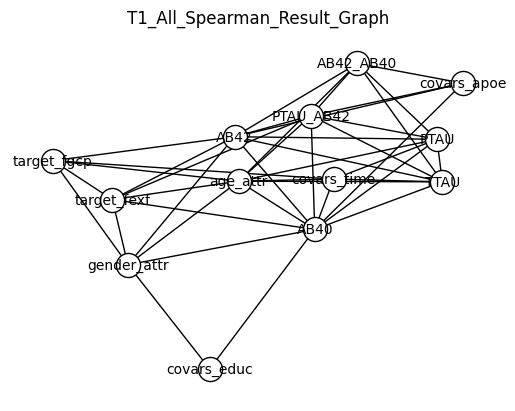
\includegraphics[width=0.24\textwidth]{diss/7_cond/figs/T1_All_Spearman_Result_Graph.png}
    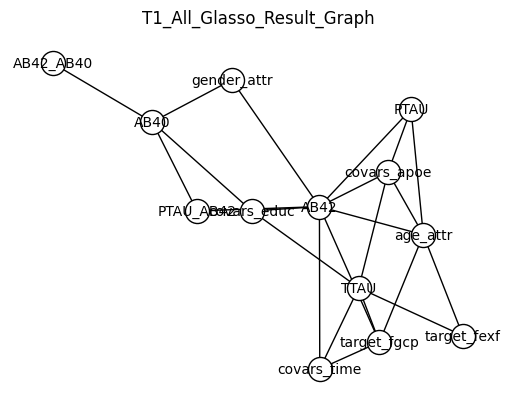
\includegraphics[width=0.24\textwidth]{diss/7_cond/figs/T1_All_Glasso_Result_Graph.png}
    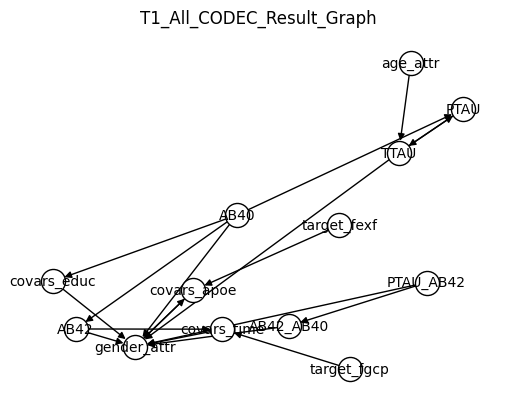
\includegraphics[width=0.24\textwidth]{diss/7_cond/figs/T1_All_CODEC_Result_Graph.png}
    \caption{All Sites.}
    \label{fig:all}
\end{figure}

\begin{figure}
    \centering
    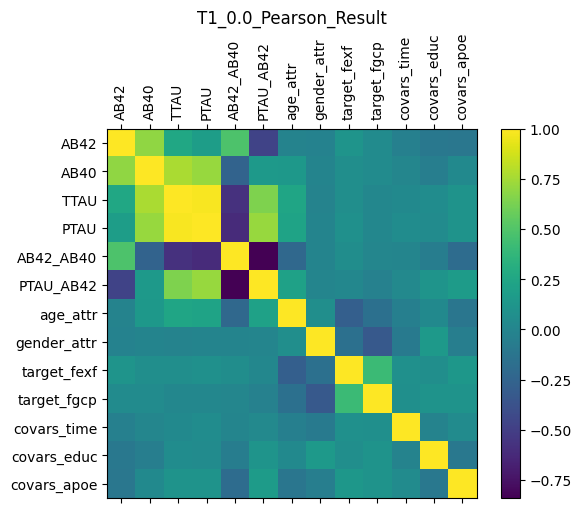
\includegraphics[width=0.24\textwidth]{diss/7_cond/figs/T1_0.0_Pearson_Result.png}
    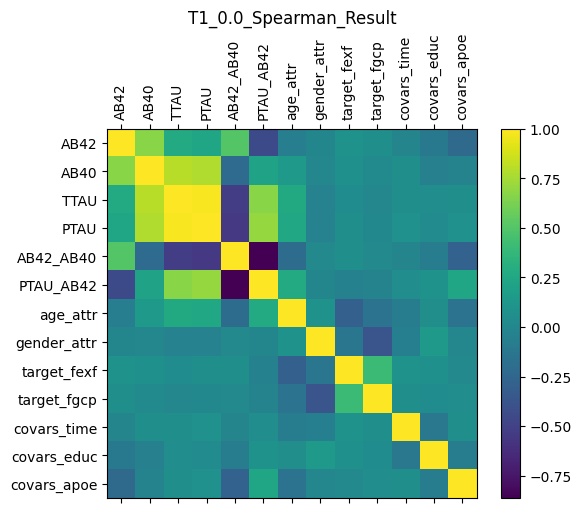
\includegraphics[width=0.24\textwidth]{diss/7_cond/figs/T1_0.0_Spearman_Result.png}
    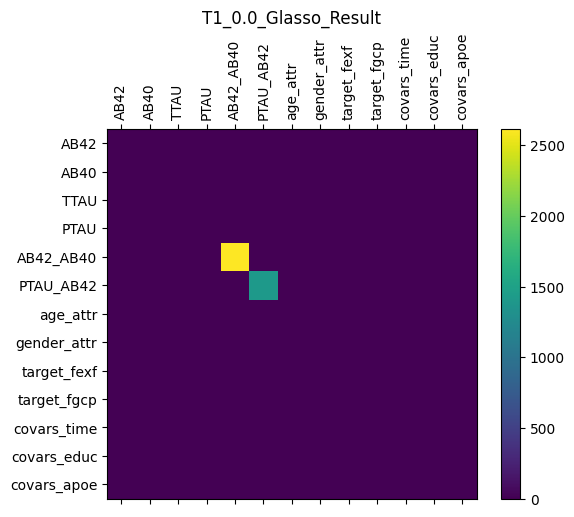
\includegraphics[width=0.24\textwidth]{diss/7_cond/figs/T1_0.0_Glasso_Result.png}
    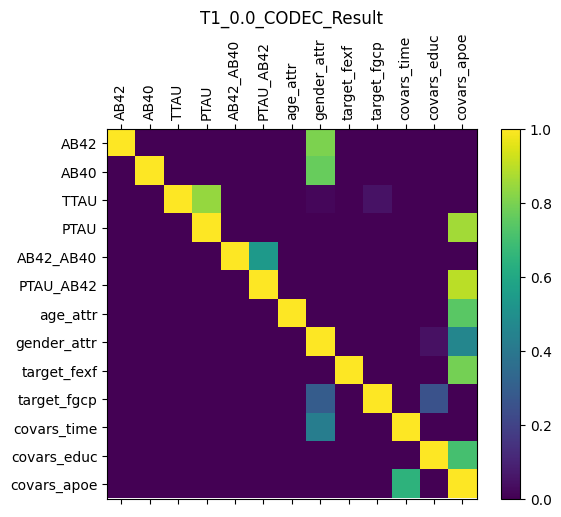
\includegraphics[width=0.24\textwidth]{diss/7_cond/figs/T1_0.0_CODEC_Result.png}
    
    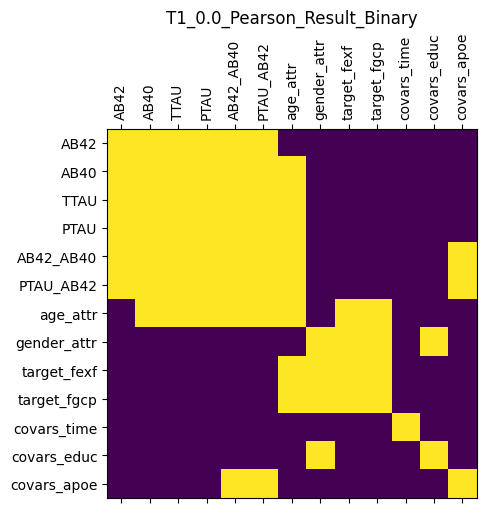
\includegraphics[width=0.24\textwidth]{diss/7_cond/figs/T1_0.0_Pearson_Result_Binary.png}
    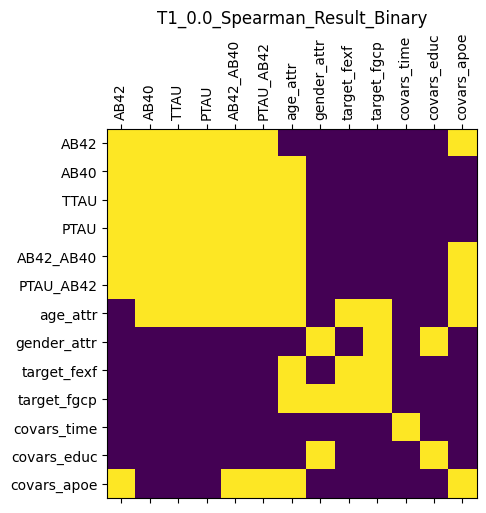
\includegraphics[width=0.24\textwidth]{diss/7_cond/figs/T1_0.0_Spearman_Result_Binary.png}
    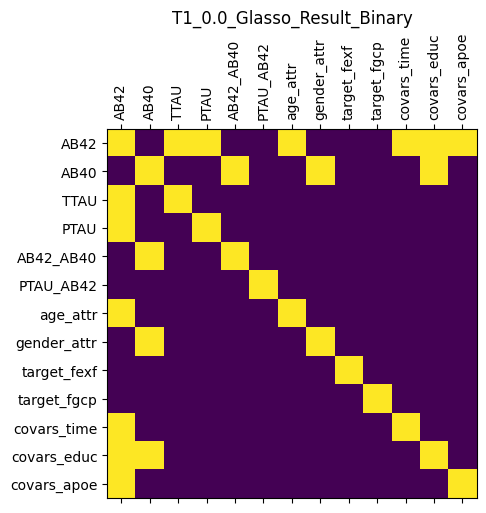
\includegraphics[width=0.24\textwidth]{diss/7_cond/figs/T1_0.0_Glasso_Result_Binary.png}
    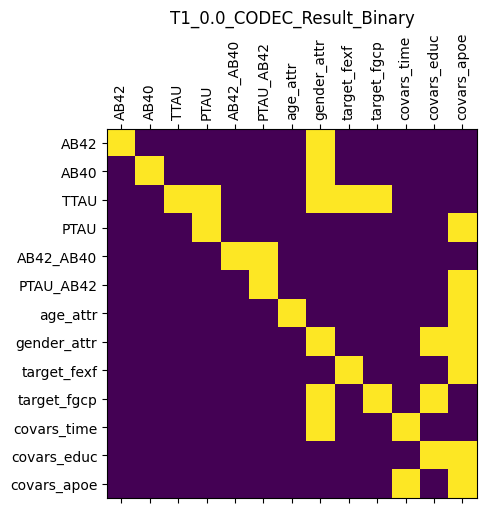
\includegraphics[width=0.24\textwidth]{diss/7_cond/figs/T1_0.0_CODEC_Result_Binary.png}
    
    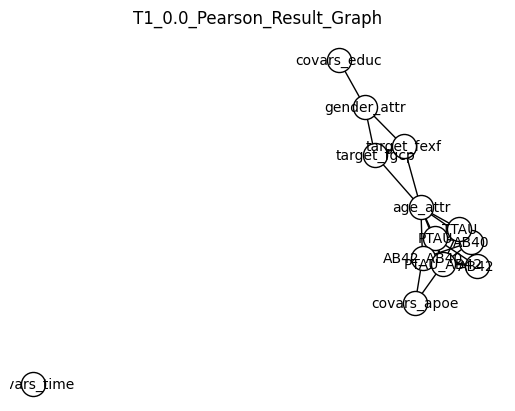
\includegraphics[width=0.24\textwidth]{diss/7_cond/figs/T1_0.0_Pearson_Result_Graph.png}
    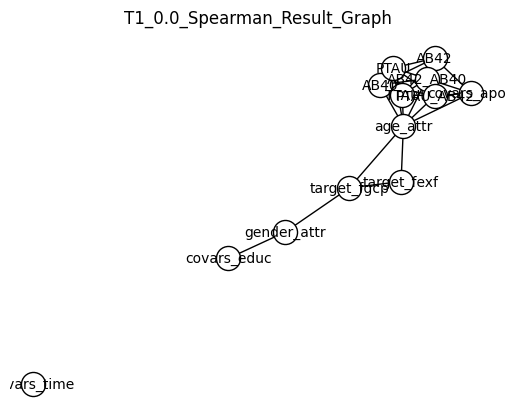
\includegraphics[width=0.24\textwidth]{diss/7_cond/figs/T1_0.0_Spearman_Result_Graph.png}
    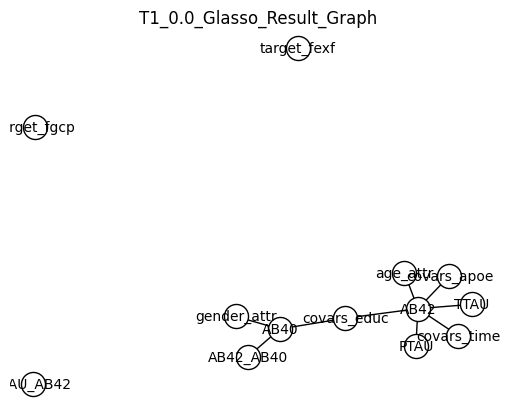
\includegraphics[width=0.24\textwidth]{diss/7_cond/figs/T1_0.0_Glasso_Result_Graph.png}
    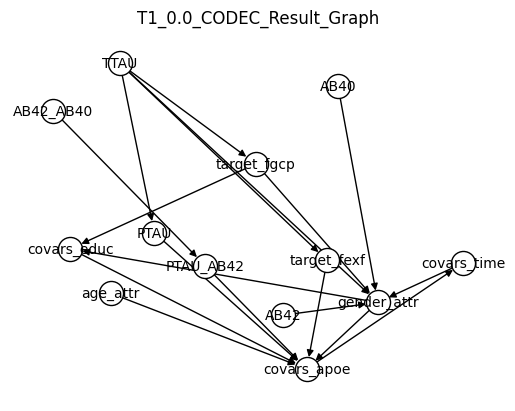
\includegraphics[width=0.24\textwidth]{diss/7_cond/figs/T1_0.0_CODEC_Result_Graph.png}
    \caption{Site 0: WRAP.}
    \label{fig:site0}
\end{figure}

\begin{figure}
    \centering
    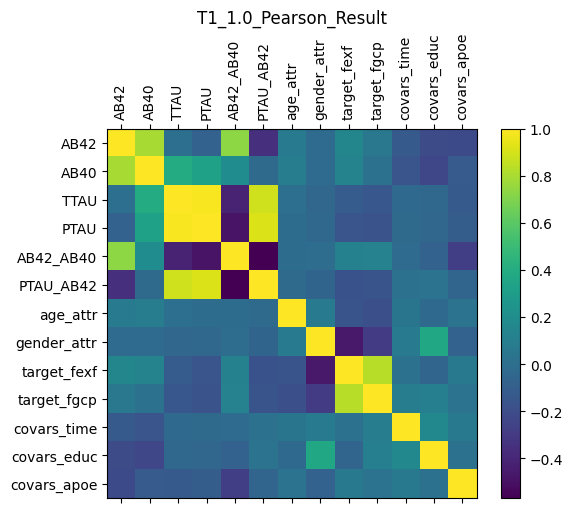
\includegraphics[width=0.24\textwidth]{diss/7_cond/figs/T1_1.0_Pearson_Result.png}
    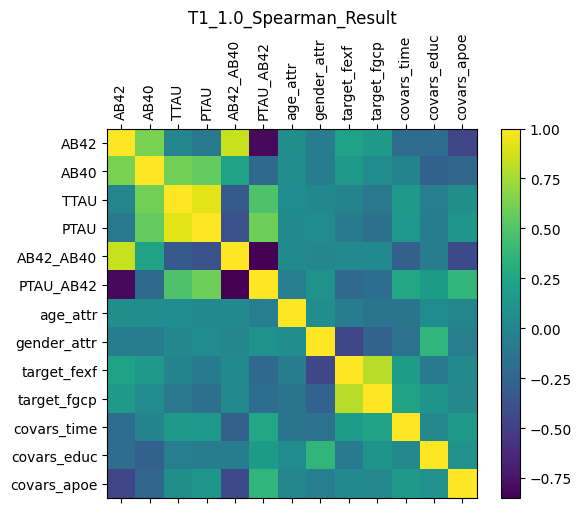
\includegraphics[width=0.24\textwidth]{diss/7_cond/figs/T1_1.0_Spearman_Result.png}
    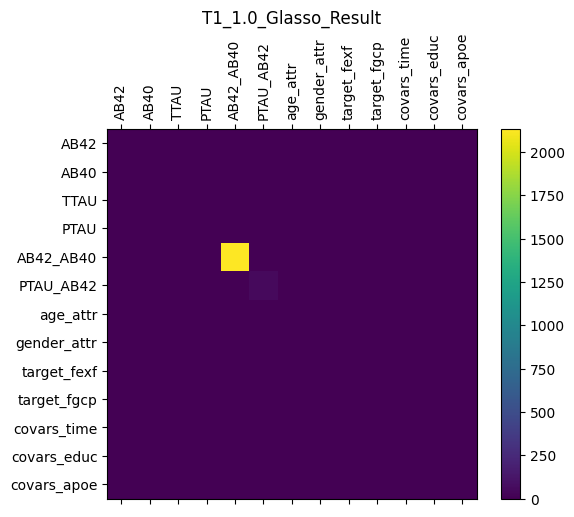
\includegraphics[width=0.24\textwidth]{diss/7_cond/figs/T1_1.0_Glasso_Result.png}
    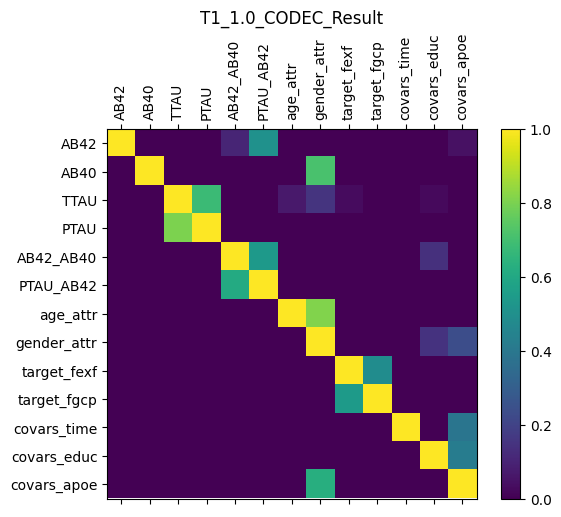
\includegraphics[width=0.24\textwidth]{diss/7_cond/figs/T1_1.0_CODEC_Result.png}
    
    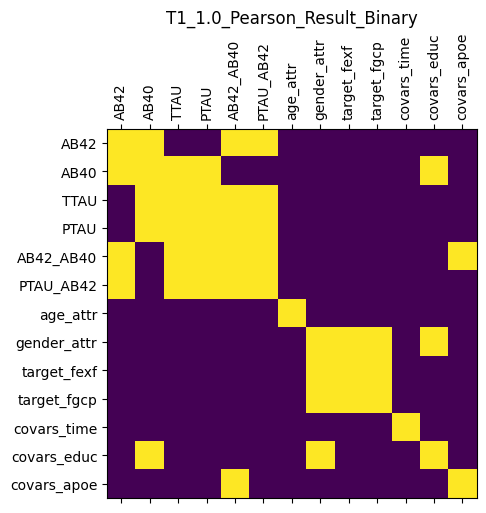
\includegraphics[width=0.24\textwidth]{diss/7_cond/figs/T1_1.0_Pearson_Result_Binary.png}
    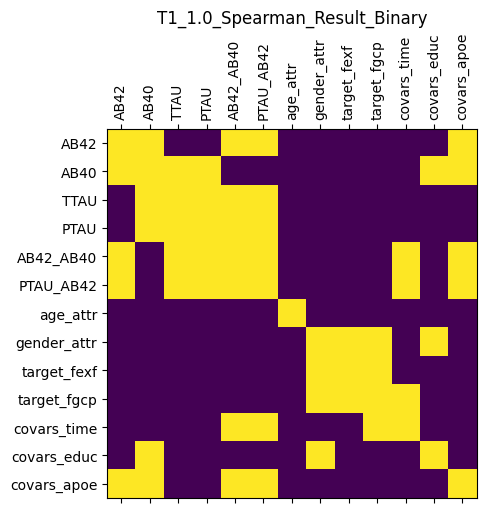
\includegraphics[width=0.24\textwidth]{diss/7_cond/figs/T1_1.0_Spearman_Result_Binary.png}
    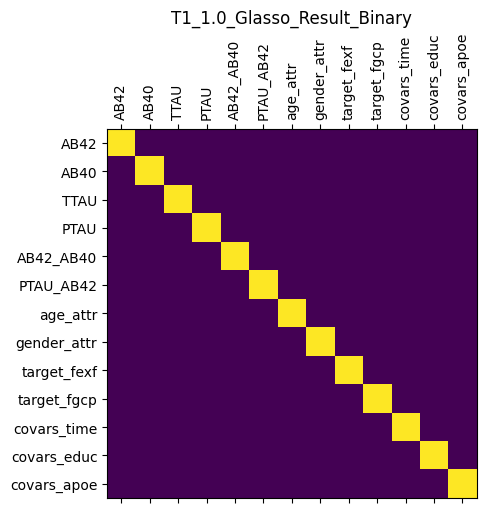
\includegraphics[width=0.24\textwidth]{diss/7_cond/figs/T1_1.0_Glasso_Result_Binary.png}
    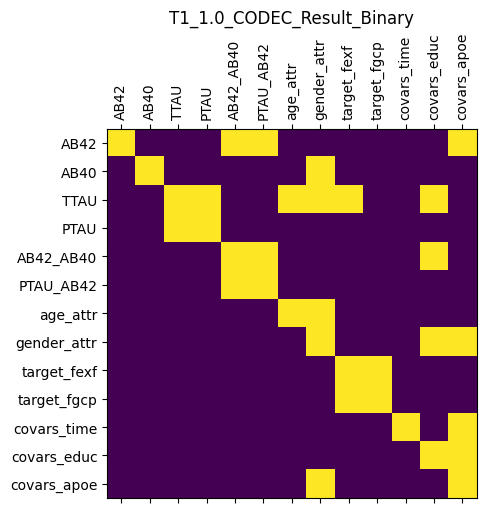
\includegraphics[width=0.24\textwidth]{diss/7_cond/figs/T1_1.0_CODEC_Result_Binary.png}
    
    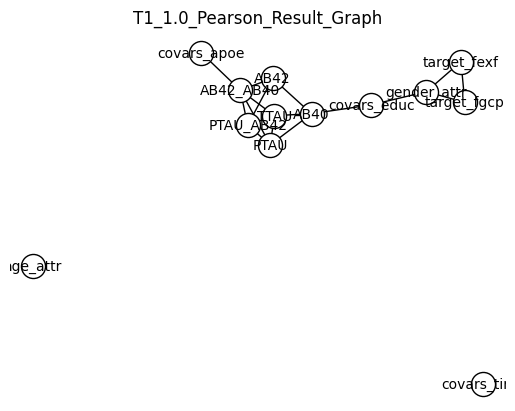
\includegraphics[width=0.24\textwidth]{diss/7_cond/figs/T1_1.0_Pearson_Result_Graph.png}
    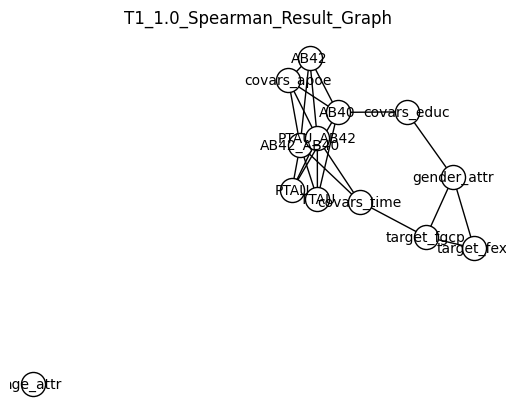
\includegraphics[width=0.24\textwidth]{diss/7_cond/figs/T1_1.0_Spearman_Result_Graph.png}
    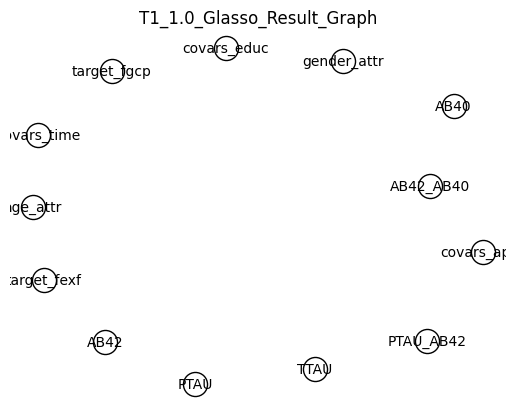
\includegraphics[width=0.24\textwidth]{diss/7_cond/figs/T1_1.0_Glasso_Result_Graph.png}
    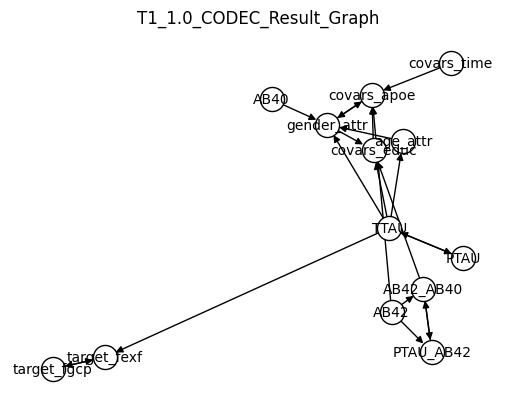
\includegraphics[width=0.24\textwidth]{diss/7_cond/figs/T1_1.0_CODEC_Result_Graph.png}
    \caption{Site 1: ACS.}
    \label{fig:site1}
\end{figure}

\begin{figure}
    \centering
    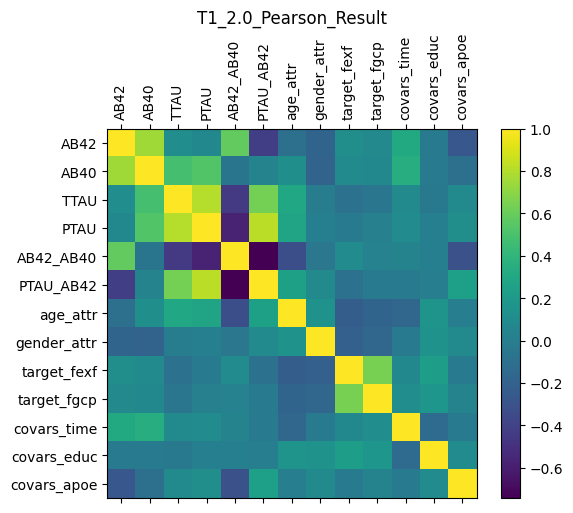
\includegraphics[width=0.24\textwidth]{diss/7_cond/figs/T1_2.0_Pearson_Result.png}
    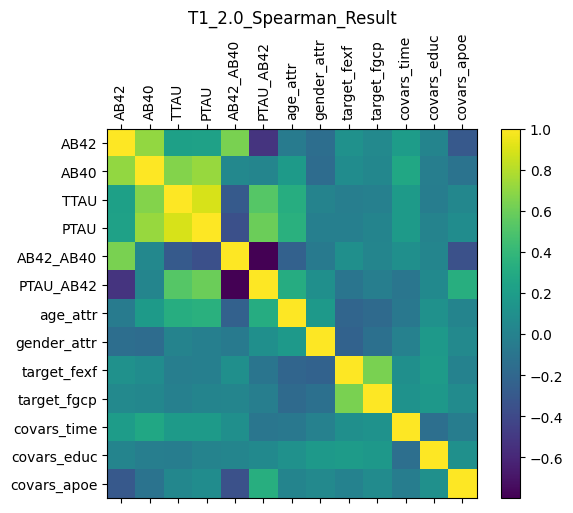
\includegraphics[width=0.24\textwidth]{diss/7_cond/figs/T1_2.0_Spearman_Result.png}
    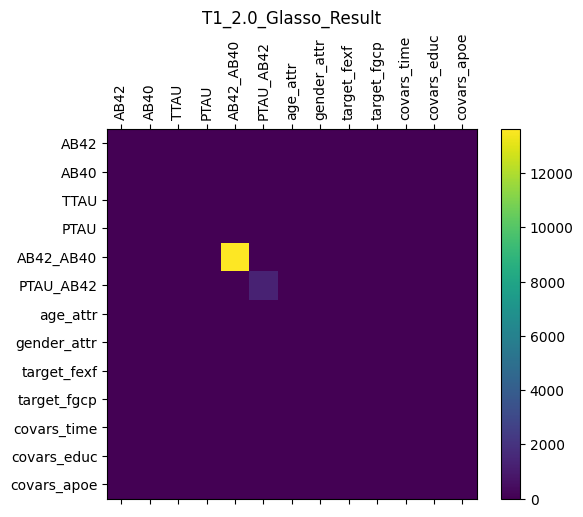
\includegraphics[width=0.24\textwidth]{diss/7_cond/figs/T1_2.0_Glasso_Result.png}
    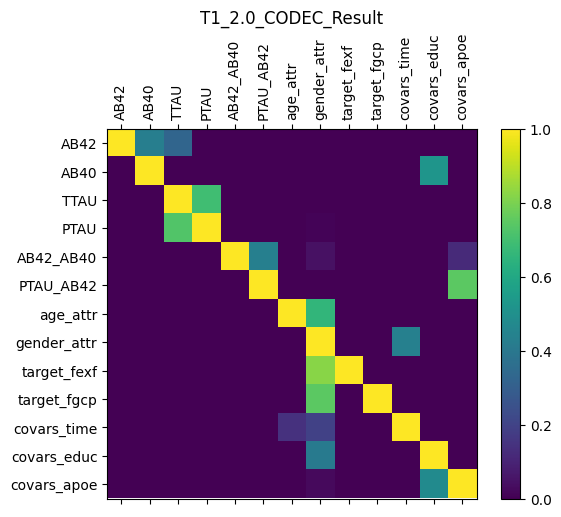
\includegraphics[width=0.24\textwidth]{diss/7_cond/figs/T1_2.0_CODEC_Result.png}
    
    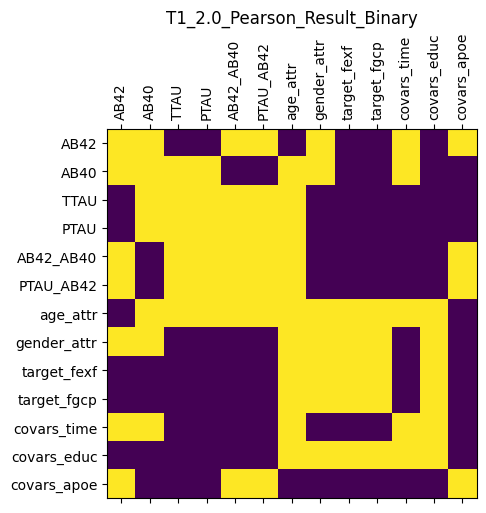
\includegraphics[width=0.24\textwidth]{diss/7_cond/figs/T1_2.0_Pearson_Result_Binary.png}
    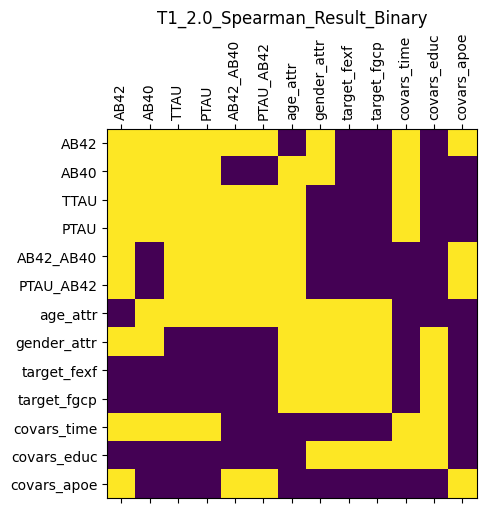
\includegraphics[width=0.24\textwidth]{diss/7_cond/figs/T1_2.0_Spearman_Result_Binary.png}
    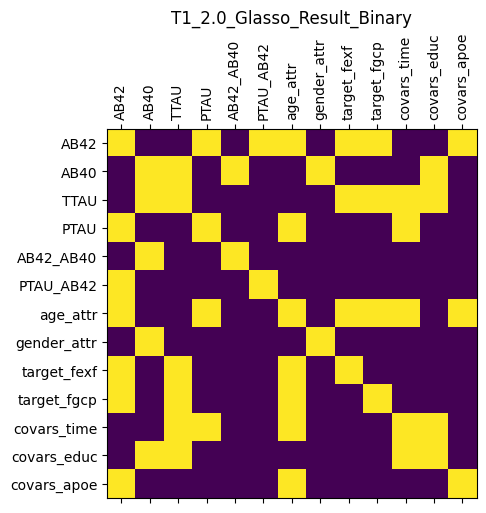
\includegraphics[width=0.24\textwidth]{diss/7_cond/figs/T1_2.0_Glasso_Result_Binary.png}
    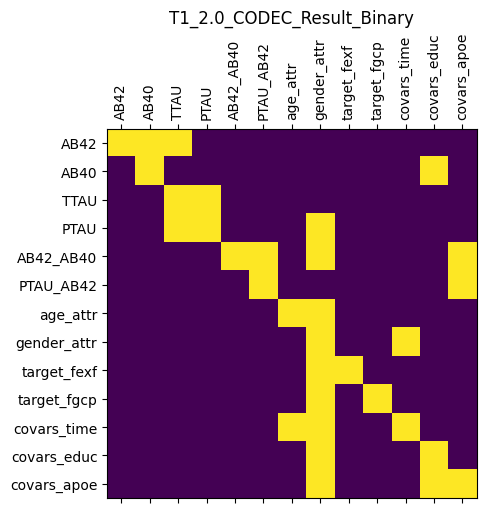
\includegraphics[width=0.24\textwidth]{diss/7_cond/figs/T1_2.0_CODEC_Result_Binary.png}
    
    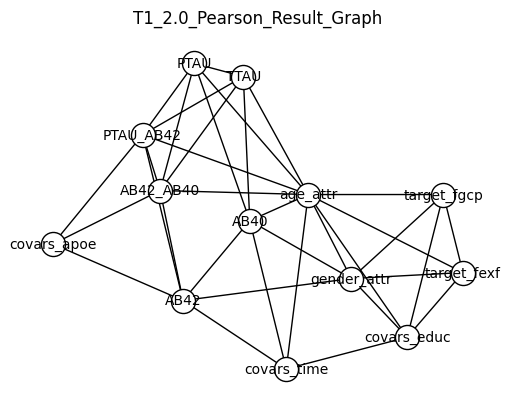
\includegraphics[width=0.24\textwidth]{diss/7_cond/figs/T1_2.0_Pearson_Result_Graph.png}
    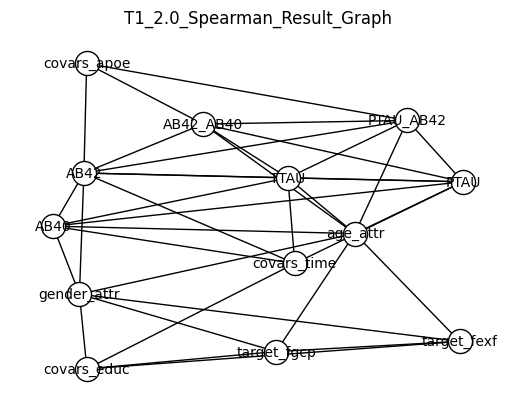
\includegraphics[width=0.24\textwidth]{diss/7_cond/figs/T1_2.0_Spearman_Result_Graph.png}
    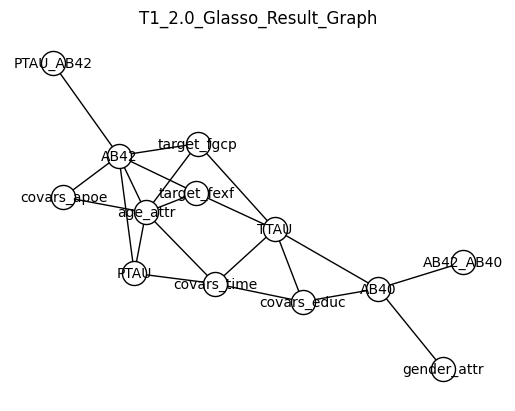
\includegraphics[width=0.24\textwidth]{diss/7_cond/figs/T1_2.0_Glasso_Result_Graph.png}
    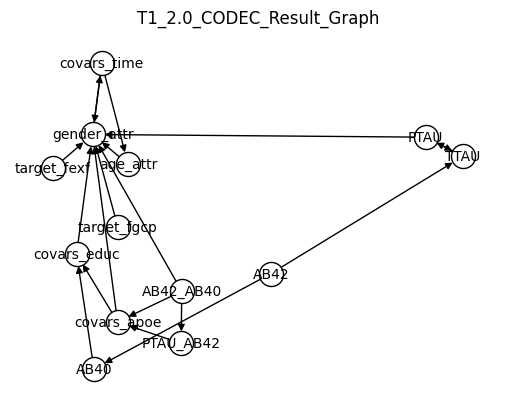
\includegraphics[width=0.24\textwidth]{diss/7_cond/figs/T1_2.0_CODEC_Result_Graph.png}
    \caption{Site 2: BIOCARD.}
    \label{fig:site2}
\end{figure}

\paragraph{Upcoming Analysis.} Future analysis will be focused on exploring the differences observed in the sparsity and conditional independences across different studies within the consortium data, as well as applying the construction longitudinally. Particular care will be taken in defining discrete timepoints, as disease progression has no predefined domain measure, and individuals within the study may be different ages at study times, as well as visiting at irregular intervals.

\section{Orthogonal Tensor Trains}\label{sec:ott}
As described in Chapter~\ref{chap:bknd}, a number of TT operations with respect to approximation and projection require computing the QR decomposition of matricized cores. In the applications for which tensor trains were originally developed, these operations were necessary \citep{oseledets2011tensor,klus2018tensor}. For modern neural network applications, where the tensor operator may be our target of learning, it may be sufficient to treat each matrix product as its own variable, and through the standard TT decomposition learn the cores along the \textbf{product of Stiefels}.

A na\"ive approach may orthogonalize the reshaped cores, and progressively push the upper triangular part of the core decomposition into the next core, resulting in the following exact formulation with appropriate reshaping:
\begin{align}
%    X(x_1,\ldots,x_d) &= A_1(x_1)\cdots A_d(x_d) \\
    \cX &= A_1^L A_2^L\cdots A_d^L \nonumber\\
    &= Q_1^L R_1 A_2^L \cdots A_d^L = Q_1^L \left(R_1 A_2^L\right) \cdots A_d^L \nonumber\\ 
    &= Q_1^L Q_2^L R_2 \cdots A_d^L \nonumber\\
    &= Q_1^L \cdots Q_d^L R_d \label{eq:eott}
\end{align}
where $ [Q_1^L, R_1] = qr(A_1^L) $, $ [Q_i^L, R_i] = qr(R_{i-1} A_i^L ), \ i \in \left \{2,\ldots,d \right \}$, and $ Q_i^L \in \RR^{r_{i-1} n_i \times r_i} \ ,\ R_i \in \RR^{r_i \times r_i} $. 
Each $Q_i^L$ is on a Stiefel given by $\ST(r_i, r_{i-1}n_i)$. Here, the number of components in the product space of Stiefels is $d$, with the `residual' $R_d \in \RR$. This decomposition is exact and only requires a reshaping of the tensor cores.
If all $r_i = r, n_i = n$,
then the total number of parameters needed is
 % the number of parameters becomes 
%is $ d n r^2 - (d-1)\frac{r^2 + r}{2}$,
%\begin{align*}
%    &=\sum_{i=1}^d \left[nr^2 - \frac{r(r + 1)}{2}\right] + \frac{r(r+1)}{2} \\
%    &= d n r^2 - d\frac{r(r + 1)}{2} + \frac{r(r+1)}{2} \\
$    d n r^2 - (d-1)\frac{r^2 + r}{2},$
%\end{align*}
%\begin{align}
%    \sum_{i=1}^d \left[r_{i-1}n_i r_i - \frac{r_i(r_i + 1)}{2}\right] + \frac{r_d(r_d+1)}{2}
%\end{align}
compared to the full format with $dnr^2$ total parameters.
It is important to note that in this formulation, the cores themselves are \textbf{not} orthogonal. Reshaping is required to bring the matricized form back to TT-cores of size $r_{i-1} \times r_i$, and in practice it is not easy to perform simple TT-tensor multiplication in this form. Additionally, we now need to optimize over Stiefel manifolds of a larger size, namely $O(nr^2)$.

\subsection{A Nicer Tensor Train Approximation}
Ideally, we would prefer a construction which keeps the standard TT-core format and involves optimization over ``smaller'' Stiefel manifolds. Consider the following representation, in which each TT-core itself is orthogonal.
\begin{definition}\label{def:ott}(Orthogonal Tensor Train)
The Orthogonal Tensor Train is defined as
\begin{align}
\cX(x_1,\ldots,x_d) = Q_1(x_1) \cdots Q_d(x_d),
\end{align}
where each $Q_i(x_i)$ lies on the Stiefel $\ST(m_i, M_i)$, where $m_i = \min(r_{i-1},r_i), \ M_i = \max(r_{i-1},r_i)$.
\end{definition}
While in this formulation the total number of components in the product space of Stiefels is $nd$, the dimension of each manifold is \textbf{significantly smaller},
dependent {\em only} on the core rank as opposed to the mode size.
The total number of parameters, if $n_i =n, r_i = r$, is
\begin{align}
n \sum_{i=1}^d \left[ r^2 - \frac{r^2 + r}{2}\right] = d n r^2 - dn\frac{r^2 + r}{2}.
\end{align}
When compared to the full TT representation,
the Orthogonal Tensor Decomposition (OTT) requires
$(r+1)/2r \approx 1/2$ as many parameters.
If $r_i=r_{i+1}$, then $\ST(m_i, M_i) = SO(m_i)$, where $SO$ is the special orthogonal group.

This construction can be seen as an approximation to the full tensor train format, in which the upper triangular part of each core is set to identity:
\begin{align}
    &\cX(x_1,\ldots,x_d) = A_1(x_1)\cdots A_d(x_d) \nonumber\\ &= Q_1(x_1)R_1(x_1)\cdots Q_d(x_d)R_d(X_d) \nonumber\\
    &\approx Q_1(x_1) \cdots Q_d(x_d)
    %&= \sum_{r_0}\cdots\sum_{r_d} A_1(x_1)[r_0,r_1]\cdots A_d(x_d)[r_{d-1},r_d] \\
\end{align}

%\begin{remark}
\paragraph{Is this useful?} It is not obvious that this construction is useful at all. How much is lost through this approximation? What is gained by using this construction? In what follows, we demonstrate that we can approximate any tensor with bounded norm using an OTT, and that with a full rank assumption and a trainable constant, our formulation admits a solution with $\epsilon$ error.
\begin{algorithm}
	\SetAlgoLined
	\For{t=1,\ldots,T}{
		$g_t := \frac{df}{d\cW} f(X^{mini-batch})$
		\For{Core $Q^i_t \in \cW_t$ and Core Gradient $g^i_t \in g_t$}{
			$G^i_t = P_{T_{\cW_t}M}(g^i_t)$ \Comment{Projection Step} \\
			$Q^i_{t+1} \leftarrow \Exp(Q^i_t, G^i_t)$ \Comment{Retraction Step}
		}
	}
	\caption{\label{alg:ott_opt} Stochastic OTT Optimization}
\end{algorithm}
\begin{figure}
	\centering
	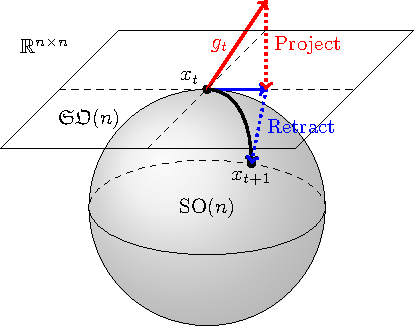
\includegraphics[width=0.75\columnwidth,trim={0 1.5cm 0 0},clip]{4_ott/figs/stiefel/stiefel_update.pdf}
	\caption{\label{fig:ott_opt} Gradient descent algorithm using the projection and retraction on the Stiefel manifold. The update is applied to each core individually, allowing for smaller manifold operations that would otherwise scale poorly with dimension.}
\end{figure}

\subsection{Theoretical Analysis}
We start by reshaping any tensor $\cX$ to a matrix $X^M$ by grouping the modes into two groups, $X^M \in \RR^{n \times m}$. We may fix this arbitrary matrix as $X^M = A \in \RR^{n \times m}$.

\begin{proposition}
\label{theory:prop1}
Given a 2D tensor $A\in \RR^{m\times m}$, $A_{ij} \in [-1,1]$, there exists sets of unit vectors, $\left\{\mathbf{x}_i\right\}_{i=1}^m\subset \RR^m$, $\left\{\mathbf{y}_j\right\}_{j=1}^m\subset \RR^m$ such that, $\forall \epsilon > 0$, $\|A - \widetilde{A}\| < \epsilon$, where, $\forall i,j,\: \widetilde{A}_{ij}=\mathbf{x}_i^t\mathbf{y}_j$.
\end{proposition}
\begin{proof}
  Let $A=USV^T$ be the SVD of $A$. Let $\epsilon > 0$, we will perturb $S$ along the diagonal to generate $\widetilde{S}$ such that, $\|S - \widetilde{S}\| < \epsilon$. Let $X=\left[\mathbf{x}_i\right]$ and $Y=\left[\mathbf{y}_i\right]$. We will first give an algorithm to generate $\widetilde{X}$ and $\widetilde{Y}$ with each
  of its column being orthonormal such that, $\widetilde{X}^T\widetilde{Y}=S$. Then, $X=\widetilde{X}U^T$ and $Y=\widetilde{Y}V^T$. 

We begin with an algorithm for $m=3$. Choose $\left\{\widetilde{\mathbf{x}}_i\right\}$ to be unit vectors and assign $\widetilde{\mathbf{y}}_3=\widetilde{\mathbf{x}}_1\times \widetilde{\mathbf{x}}_2$, $\widetilde{\mathbf{y}}_2=\widetilde{\mathbf{x}}_3\times \widetilde{\mathbf{x}}_1$. Then, make $\widetilde{\mathbf{y}}_2$ and $\widetilde{\mathbf{y}}_3$ to be of unit length. %Clearly, $\widetilde{\mathbf{x}}_2^t\widetilde{\mathbf{y}}_2\neq 0$ and $\widetilde{\mathbf{x}}_3^t\widetilde{\mathbf{y}}_3\neq 0$. 
Now, rotate $\widetilde{\mathbf{x}}_2$ in the plane spanned by $\left\{\widetilde{\mathbf{x}}_1, \widetilde{\mathbf{x}}_2\right\}$ such that,
$\widetilde{\mathbf{x}}_2^t\widetilde{\mathbf{y}}_2=\widetilde{S}_{22}$. Similarly, rotate $\widetilde{\mathbf{x}}_3$ in the plane spanned by $\left\{\widetilde{\mathbf{x}}_3, \widetilde{\mathbf{x}}_1\right\}$ such that,
$\widetilde{\mathbf{x}}_3^t\widetilde{\mathbf{y}}_3=\widetilde{S}_{33}$. Now, assign, $\widetilde{\mathbf{y}}_1=\widetilde{\mathbf{x}}_2\times \widetilde{\mathbf{x}}_3$ and make it unit length. Now, fixing $\widetilde{\mathbf{x}}_2$ and $\widetilde{\mathbf{x}}_3$, the above steps are a continuous mapping, $F$ from $\mathbf{S}^2$ to $[-1,1]$, i.e., by changing different $\widetilde{\mathbf{x}}_1 \in \mathbf{S}^2$, we will get different values for $\widetilde{\mathbf{x}}_1^t\widetilde{\mathbf{y}}_1$. Also, notice that, if, for a particular choice of $\left\{\widetilde{\mathbf{x}}_i\right\}$, $\widetilde{\mathbf{x}}_1^t\widetilde{\mathbf{y}}_1>0$, then, for the choice of $\left\{\widetilde{-\mathbf{x}}_i\right\}$, the above construction returns $-\widetilde{\mathbf{y}}_2$ and $-\widetilde{\mathbf{y}}_3$ and $F$ returns, $-\widetilde{\mathbf{x}}_1^t\widetilde{\mathbf{y}}_1<0$. Thus if $a \in F\left(\mathbf{S}^2\right)$,  $-a \in F\left(\mathbf{S}^2\right)$. Furthermore, $1\in F\left(\mathbf{S}^2\right)$ and hence, $-1\in F\left(\mathbf{S}^2\right)$. As $\mathbf{S}^2$ is connected and $F$ is continuous,
$F\left(\mathbf{S}^2\right)$ is connected, and so, $\exists$ $\left\{\mathbf{x}_i\right\}_{i=1}^m\subset \RR^m$ and $\left\{\mathbf{y}_j\right\}_{j=1}^m\subset \RR^m$, s.t., $\left(\forall \left\{i, j\right\}\right)$, 
$\widetilde{\mathbf{x}}_i^t\widetilde{\mathbf{y}}_j = \widetilde{S}_{ij}$. Since $\|S-\widetilde{S}\|< \epsilon$ and the
choice of $\epsilon> 0$ is arbitrary, we can see that $\|A - \widetilde{A}\| < \epsilon$.

Using the generalization of cross product by exterior algebra, the above procedure can be naturally extended to arbitrary $m>3$.
\end{proof}

A direct corollary of the above result allows approximating an arbitrary 2D matrix,
\begin{corollary}\label{theory:corr1}
Given a 2D tensor $A \in \RR^{m \times m}$, there exists sets of unit vectors, $\left\{\mathbf{x}_i\right\}_{i=1}^m\subset \RR^m$, $\left\{\mathbf{y}_j\right\}_{j=1}^m\subset \RR^m$ and fixed constant $c$ such that, $\forall \epsilon > 0$, $\|A-\widetilde{A}\|< \epsilon$, where, $\forall i,j,\: \widetilde{A}_{ij}=c\mathbf{x}_i^t\mathbf{y}_j$.
\end{corollary}
\begin{proof}
Given any arbitrary matrix $A$, define $A^\prime = A/|A|_{\infty}$. Then $A^\prime_{ij} \in [-1,1]$, and by Proposition \ref{theory:prop1} we can construct unit vectors $\textbf{x}_i,\textbf{y}_j$ such that $\forall \epsilon > 0$, $\|A^\prime_{ij} - \textbf{x}_i^T\textbf{y}_j\|< \epsilon$. Then immediately $\forall A_{ij}$, we have $A_{ij} = cA^\prime_{ij}$ where $c = |A|_\infty$.
\end{proof}

We also have the following directly from Proposition \ref{theory:prop1}.
%%%%%%%%%%% matrix vector
\begin{corollary}\label{theory:corr2}
Given a 2D tensor $A\in \RR^{m\times m}$, with $\|A\|_F\leq 1$, there exists a set of orthonormal matrices $\left\{B_i\right\} \subset SO(m)$ and a set of unit vectors $\left\{\mathbf{y}_j\right\}_{i=1}^m\subset \RR^m$ such that $\forall \epsilon > 0$, $\|A - \widetilde{A}\|< \epsilon$, where, $\forall i,j,\: \widetilde{A}_{ij}= \mathbf{1}^t B_i^t\mathbf{y}_j$.
\end{corollary}
%\begin{proof}
%The proof follows from Proposition \ref{theory:prop1}.
%\end{proof}

\begin{example}Applying the above result to OTT, equivalence is relatively straightforward to show. 
%\begin{example}
Consider the problem of approximating a 4 dimensional tensor $\cX$ with $n_{1,2,3,4}=n=r$. Let $Q_1(x_1) \in \RR^{1\times n}, Q_2(x_2), Q_3(x_3) \in \RR^{n \times n}$, and $Q_4(x_4) \in \RR^{n \times 1}$. By Corollary \ref{theory:corr2} we can write two vectors indexed by $x_1,x_2$ and $x_3,x_4$ as $X^A (x_1,x_2) = Q_1(x_1)^\top Q_2(x_2)$ and  $X^B(x_3,x_4) = Q_3(x_3)Q_4(x_4)$ respectively. The multiplication of these vectors $X^A,X^B$ again yields a single element indexed by $x_1,x_2,x_3,x_4$, which can take any value between $[-1,1]$ by Proposition \ref{theory:prop1}. Then clearly the cores $Q$ form an equivalent definition of $\cX$.
%\end{example}
\end{example}

We can then apply Corollary \ref{theory:corr2} and find that the product of indexed orthonormal matrices and orthonormal vectors with full rank can approximate any matrix with bounded norm. 
Applying this to our OTT format, it immediately follows that with  the addition of at most $dn$ constants in $\RR$ we can approximate any arbitrary tensor. While this addition would put the format well over the number of parameters in the standard format, this provides sufficient evidence that, in typical learning settings in which our model is already overparameterized, we can still capture the full expressive power of the model class in which an OTT format is inserted. 

{\bf Remark.} It also important to note that the above calculation of dimensionality is the \textit{intrinsic} dimension. The number of actual allocated variables is indeed $dn^3$ for an exact formulation.
It remains open to theoretically analyze the degradation of the approximation as $r<n$.

\subsection{Efficient Stiefel Optimization}\label{sec:opt}
Here, we describe how to compute an OTT approximation of a tensor $\cW$, which can be posed as the following minimization problem.
\vspace{-5pt}
\begin{align}
\min_{\left\{Q_i(x_i)\right\}_{i=1}^d} E &= \sum_{\left\{x_i\right\}} \|\cW(x_1,\ldots,x_d) - Q_1(x_1)\cdots Q_d(x_d)\| \notag \\ \quad & \mbox{s.t.} \quad Q_i(x_i)^\top Q_i(x_i) = I_p \quad \forall i, x_i
\end{align}
Notice that this optimization is difficult because of the orthogonality constraint \cite{edelman1998geometry,collins2014spectral}. An efficient way to solve this is by doing the optimization on the product of (compact) Stiefel manifolds: let it be denoted by $\mathcal{P}_S$. We will use the product $\ell_2$ metric on this product space. Given $x_1, \cdots x_d$, we perform
an optimization on the product of Stiefel manifolds to solve for $\{Q_i(x_i)\}$ for $i\in[1\ldots d]$. We use a Riemannian gradient descent technique on this product of Stiefel manifolds $\mathcal{P}_S$. Given $\{Q^t_i(x_i)\}$ as the solution of the $t^{th}$ step, the $(t+1)^{th}$ solution, $\{Q^{t+1}_i(x_i)\}$, can be computed using 
\vspace{-5pt}
\begin{equation}
\left\{Q^{t+1}_i(x_i)\right\} = \text{Exp}\left(\left\{Q^{t}_i(x_i)\right\}, \frac{\partial E}{\partial \left\{Q^{t}_j(x_j)\right\}}\right),
\end{equation}
where $\text{Exp}$ is the Riemannian Exponential map on $\mathcal{P}_S$. On $\mathcal{P}_S$, computation of Riemannian Exponential map is not tractable and needs an optimization, hence we
use a Riemannian retraction map as proposed in \cite{6340355}.

Figure \ref{fig:ott_opt} summarizes this procedure. For each orthogonal core, the gradient is computed with respect to the Euclidean ambient space and projected to the tangent space at the current iterate. The update is constructed by moving back to the Stiefel with the Riemannian exponential map.

\subsection{Square Stiefels/SO(n)}
In practice, when learning an OTT operator, we will primarily be setting the rank to be fixed for all cores.
The Stiefel manifold, $\ST(n,n)$ with $n=p$ is equal to the special orthogonal group $\text{SO}(n)$.
The Riemannian Exponential map on $\text{SO}(n)$ is the matrix exponential, computationally intensive to both compute and backpropagate through.
Hence, we use the Cayley map from $\mathfrak{SO}(n)$ to $\text{SO}(n)$, given by $A \mapsto \left(I-A\right)\left(I+A\right)^{-1}$, where $\mathfrak{SO}(n)$ (the space of $n\times n$ skew-symmetric matrices) is the tangent space of $\text{SO}(n)$ at identity.
Although the Cayley map requires a matrix inverse, it is much easier to handle using standard tools
in modern toolboxes (e.g., TensorFlow, PyTorch).

%\begin{wrapfigure}[]{r}{0.4\textwidth}
%\begin{figure}
%\begin{minipage}[t]{0.5\textwidth}
%			\vspace{-45pt}
%		\begin{algorithm}[H]
%			\caption*{}
%			\begin{algorithmic}
%				\Function{OTT-Core}{$r$}
%				\State $w \leftarrow \RR^{r(r-1)/2}$
%				\State $R \leftarrow \text{triu}(w)$
%				\State $A \leftarrow R - R^\top$
%				\State $Q \leftarrow (I - A)(I + A)^{-1}$
%				\State return $Q$
%				\EndFunction
%			\end{algorithmic}
%		\end{algorithm}
%%	\end{minipage}
%	\captionof{algorithm}{OTT Core.\label{alg:ott-core}}
%%	\vspace{-20pt}
%%\end{wrapfigure}
%\end{figure}

 Observe that
the work in \cite{helfrich2017orthogonal} used the Cayley map for RNNs, but does not make use of the sparse representation of a skew-symmetric matrix $A \in \mathfrak{SO}(n)$.
In contrast, in our formulation we use the Cayley map as a mapping from $\mathbb{R}^{\frac{n(n-1)}{2}}$ to $\text{SO}(n)$. This enables a strict reduction in the number of trainable/learnable variables in a network, and provides a direct path through which gradients can be computed and backpropagated.
Algorithm \ref{alg:ottcore} describes the procedure for constructing an OTT-core.
The Euclidean variable vector $w$ is mapped directly to the upper triangular part, defined as $\triu(\cdot)$, of a new matrix $R$, and by subtracting its transpose,
we arrive at a skew symmetric matrix $A$. The Cayley map, as described above, maps to our Orthogonal OTT Core. 

\textbf{Remark.} Note that the Cayley map is not a bijective mapping between $\mathfrak{SO}(n)$ and $\text{SO}(n)$ as the range is not the entire $\text{SO}(n)$. This is because the Cayley map cannot generate matrices with negative eigenvalue(s). Empirically, we do not find this to be an issue when learning the OTT representation directly.

With this efficient approximation in hand, we are able to directly apply our OTT formulation to architectures for a variety of applications.
\iffalse
 {\begin{algorithm}[t]
 		\caption{ \label{alg:ottcore} Constructing an OTT Variable}
 		\begin{algorithmic}
 		    \Function {OTT-Variable}{$d, n_{in}, n_{out}, r$}
 		        \State $OTT \leftarrow \emptyset$
 		        \For{$i \in 1,\ldots,d$}
 		            \For{$j,k \in 1,\ldots,n_{in}[i],1,\ldots,n_{out}[i]$}
                        \State $OTT$.append(OTT-Core($r$))
                    \EndFor
 		        \EndFor
 			    \State return $OTT$
 			\EndFunction
 			\Function {OTT-Core}{$r$}
     			\State $w \leftarrow \RR^{r(r-1)/2}$
     			\State $R \leftarrow \triu(w)$
     			\State $A \leftarrow R - R^\top$
     			\State $Q \leftarrow (I - A)(I + A)^{-1}$
     			\State return $Q$
 			\EndFunction
 		\end{algorithmic}
\end{algorithm}}
\fi
\begin{figure}
	\centering
	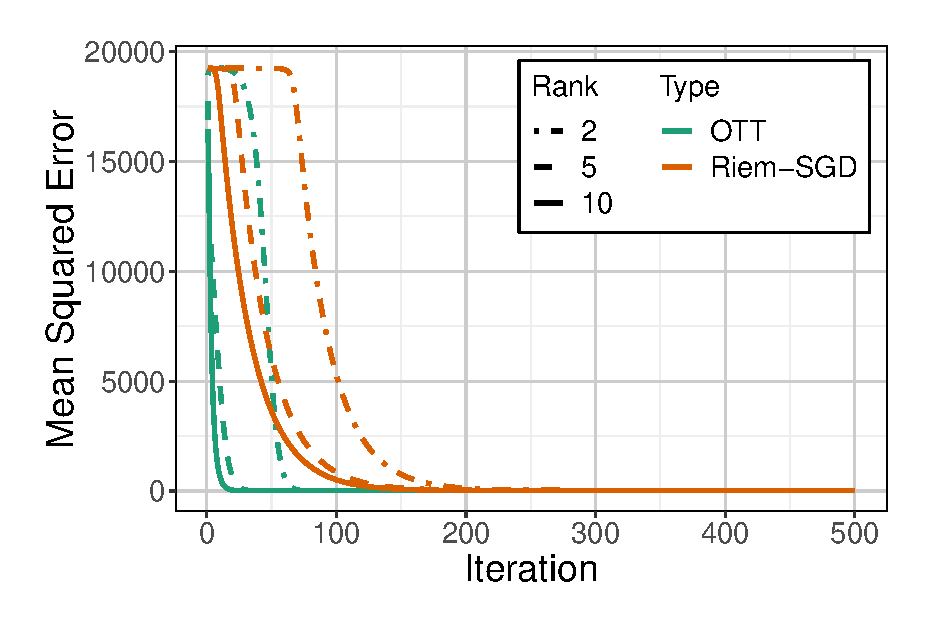
\includegraphics[width=0.32\textwidth]{4_ott/figs/sim/rank_convergence.eps}
	\includegraphics[width=0.32\textwidth]{4_ott/figs/sim/time_comparison.eps}
    \includegraphics[width=0.32\textwidth]{4_ott/figs/sim/mem_vs_rank.eps}
	\caption{\label{fig:riemstief} \footnotesize (left) Mean squared error for different TT-ranks,
          using both the Riemannian formulation \eqref{eq:riem} and the approximate Stiefel formulation \eqref{eq:eott}.
          (center) Effect of TT-rank on per iteration runtime of both methods. OTT is significantly faster (10x)
          than the Riemannian formulation.
          (right) Memory Dependence of both TT and OTT constructions as a function of rank.
          The OTT formulation allows for models roughly double the size of TT.}
\end{figure}

\section{Evaluating performance on Simulations, Moving MNIST and Video data}\label{sec:exps}
First,
we evaluate how well our OTT formulation performs relative to existing methods, on synthetic
datasets as well as other popular datasets used for sequential deep models. 
%All synthetic experiments were conducted using a Tensorflow implementation on
A Nvidia Titan Xp GPU was used. 

\textbf{(A) OTT vs Riemannian SGD on synthetic data.}
To empirically verify the claims in Section \ref{sec:ott}
and to evaluate the value of our OTT construction over the existing Riemannian SGD framework,
we simulate a simple least squares problem with the goal of learning a tensorized weight matrix,
$$\min_{W_{TT}} \sum_{i=1}^n ||y_i - W_{TT}x_i||^.2$$
Here we use the na\"ive but exact OTT construction,
using the optimization scheme in Section \ref{sec:opt}.
A weight matrix $W$ is initialized to a random matrix with size $784 \times 625$, and samples are drawn from $y=Wx$. The matrix is reshaped as a tensor with modes $[4,7,4,7] \times [5,5,5,5]$.

\paragraph{Results.} Figure \ref{fig:riemstief} shows the
convergence rates of both methods with fixed learning rates for various TT-ranks.
\textbf{(a) Quality and speed.} For this toy problem, not only is the OTT construction able to find a good solution, it is able to find it significantly faster than Riemannian SGD.
\textbf{(b) Update steps.} Additionally, we note that the time per iteration is significantly shorter for the OTT construction.
%On the hardware described the OTT method takes approximately 0.07 seconds/iteration, while the Riemannian method takes 0.38, 0.55, and 1.00 seconds per iteration for each of the TT ranks evaluated.
OTT allows for each manifold update step to be performed on a low dimensional Stiefel,
and so retraction and projection is \textit{fast.}
The Riemannian method requires left orthogonalization and QR decompositions
of larger matrices, leading to a slower, TT-rank dependent runtime, shown in Figure \ref{fig:riemstief}.
\textbf{(c) Memory footprint.} Finally, we see in Figure \ref{fig:riemstief} that the memory consumption of OTT is quite modest compared to TT (which already offers
significant memory savings over alternative existing schemes). This may be a beneficial feature
when running a large sequential model on less expensive GPUs. 
Given these results, we use a basic SGD update for TT in subsequent experiments. 

\paragraph{(B) Moving MNIST.}
The moving MNIST dataset \cite{srivastava2015unsupervised} consists of handwritten digits moving within a specified larger image.
%Designed as a toy version of video data, moving MNIST is a standard benchmark for recurrent algorithms.
We first demonstrate that
for simple sequences, reconstruction under a complete tensor train framework is possible,
and representing fully connected layers with an OTT layer
reduces the number of parameters \textbf{without} image degradation.
Here, we use a vanilla RNN, with a state size of 4096 and TT-Rank 64.
%Figure \ref{fig:ttvsottmnist} shows the outputs after 100 training epochs of 20K samples with a batch size of 32. The hidden layer was of size 1024 and TT-rank 32, for images of size $64 \times 64$. Comparing the TT and OTT results, we observe a slight difference in reconstruction quality, at the cost of a hidden layer twice as large.
%\begin{figure*}[t]
%    \centering
%    $\overbrace{\hspace{0.495\textwidth}}^{\text{OTT Reconstruction}}$ $\overbrace{\hspace{0.495\textwidth}}^{\text{TT Reconstruction}}$ \\
%    \includegraphics[width=0.49\textwidth,trim={24cm 20cm 0 0},clip]{figs/ott_epoch_99_valid_imgs.png}
%    \includegraphics[width=0.49\textwidth,trim={24cm 0 0 20cm},clip]{figs/tt_epoch_99_valid_imgs.png}
%    \caption{Reconstruction results of 3-length Moving MNIST digits with frame size 64 by 64 pixels, for both TT and OTT constructions.}
%    \label{fig:ttvsottmnist}
%\end{figure*}

\paragraph{Results.} Figure \ref{fig:256digits} shows the ground truth and reconstruction
results for images with size $256 \times 256$, where each sequence is of length 8,
and the direction and orientation of the digit is random.
\textbf{(a) Reconstruction accuracy and model size.}
The entire recurrent network is compressed with OTT layers for input-to-hidden, hidden-to-hidden,
and hidden-to-output maps. With a large state size of 4096, we are able to nicely capture and
rebuild the entire sequence with a significantly smaller model size.
\begin{figure}
    \centering
    \includegraphics[width=0.9\textwidth,trim={0 1.5cm 0 1cm},clip]{4_ott/figs/mnist/DMNIST_gt.eps}
    \includegraphics[width=0.9\textwidth,trim={0 1cm 0 1.5cm},clip]{4_ott/figs/mnist/DMNIST_pd.eps}
    \includegraphics[width=0.9\textwidth,trim={0 1.5cm 0 1cm},clip]{4_ott/figs/mnist/FMNIST_gt.eps}
    \includegraphics[width=0.9\textwidth,trim={0 1cm 0 1.5cm},clip]{4_ott/figs/mnist/FMNIST_pd.eps}
    \vspace{-10pt}
    \caption{    \label{fig:256digits} \footnotesize Sample ground truth (top) and reconstruction (bottom) of Moving MNIST digit and fashion sequences of size $256 \times 256$. We
    see good consistency between each upper/lower rows for both datasets.}
\end{figure}
\textbf{(b) Scaling to larger images.}
This effective compression also allows us to scale up --  to
significantly larger images of size $1024 \times 1024$, \textit{with no loss in reconstruction quality},
    without the need for more sophisticated convolutional architectures.

\textbf{(C) Hollywood2.}
We find
    that these results extend nicely to LSTMs/GRUs and for classification tasks
    as well. The Hollywood2 dataset \cite{marszalek09} consists of video clips from 69 movies
    labeled with 12 different actions from ``answering the phone" to ``driving a car'' (Figure \ref{fig:hollywood}).
    Following the preprocessing steps of \cite{pmlr-v70-yang17e}, we feed resized
    clips of size $234 \times 100 \times 3 \times T$ to our model, where the length of a sequence
    (number of frames) $T$ ranges from $29$ to $1496$. We tensorize the
    input as $10 \times 18 \times 13 \times 30$ for all input sequences (padded to $1496$) and the
    hidden states as $4 \times 4 \times 4 \times 4$, with TT and OTT ranks set as 4.

\textbf{Results.} Tensor trains here allow us to completely operate on the \textit{entire video sequence.}
    \textbf{(a) Parameter size.}
    The number of parameters in our model is a few thousands ($1864$ for OTT, $3104$ for TT)
    compared to millions needed for a standard fully connected model.
\textbf{ Accuracy comparison.}
    Using Mean Average Precision (MAP) as a measure of accuracy for this multi-label problem, we
    find that using an OTT-LSTM or OTT-GRU in place of a TT-LSTM or TT-GRU leads to
    \textit{no significant difference in MAP.} 
	
% Figure \ref{fig:1024digits} shows one reconstruction generated by our model on Fashion MNIST \cite{xiao2017/online}, a similar dataset in which images are of a set of 10 typical articles of clothing.
%\begin{figure}[]
%    \centering
%    \includegraphics[width=\columnwidth,trim={24cm 15cm 0 0},clip]{figs/fashion_1024.eps}
%    \caption{Reconstruction for images of size $1024 \times 1024$.}
%    \label{fig:1024digits}
%\end{figure}
%Additional high-dimensional experiments, including prediction of future frames, can be found in the supplement.

% \subsection{RNN Benchmarks}
% Copy Memory Problem, Adding Problem (straight comparison from others)

% cross entropy vs iterations for copy

% mse for adding

% \cite{helfrich2017orthogonal,arjovsky2016unitary,wisdom2016full,jing2017tunable,mhammedi2017efficient}

% scaled cayley (arxiv)

% full-urnn (wisdom)

% rc-urnn (arjovsky)

\section{Identifying Differential Progression in AD}\label{sec:adni}
\paragraph{Motivation.} The Alzheimer's Disease Neuroimaging Initiative (ADNI, \url{adni.loni.usc.edu})  provides a comprehensive dataset
targeted towards understanding AD. The goals of the initiative include measuring the development of the disease as a function of different imaging modalities, other biological markers, and clinical and neuropsychological assessments. 
Deep learning methods traditionally applied to this corpus require imaging data to be heavily preprocessed into summary measures, such as \textit{regions of interest}.
In other cases, based on the needs of the application (e.g., segmentation),
the approach may operate with 3D image patches instead of the entire image. 
The size of the images, especially when considered longitudinally, can be impractical for modern deep learning frameworks unless some novel
implementation tricks are utilized. 

\textbf{Data.} Our dataset consists of 522 subjects with Magnetic Resonance Imaging (MRI) scans collected over three years. For each individual, an MRI was collected annually, along with a battery of neuropsychological evaluations.

\textbf{Pre-processing.}
Full head MRIs were processed using SPM12 \cite{ashburner2014spm12}. Each image was segmented/registered using the MNI152 template. Gray matter probabilities were computed, and these gray matter density (GMD) images were used as input to our models.
The processed image size was $121 \times 145 \times 121$ (voxel size $1.5mm^3$), with \textbf{3 images per subject}.

\textbf{Model.} At this scale, we use convolutional input and deconvolutional output layers to incorporate local information with respect to reconstruction and prediction. The architecture consists of a straightforward 3-state RNN with input-hidden, hidden-hidden, and hidden-output layers replaced with TT and OTT layers. Input volumes are passed through a 3D convolutional input network, with max-pooling layers and ReLUs.
Hidden states are passed through an output convolutional network consisting of max-unpooling layers using indices
saved from the input CNN.
Strides were fixed at 1 with a kernel size of $3\times 3 \times 3$,
with successive convolutions decreasing (increasing) the number of channels by 2.
Max pooling was applied uniformly to all 3 input channels with a stride of 2. Adam optimization \citep{kingma2014adam} was used for all
ADNI experiments, with learning rate $1e^{-3}$, and decay rate $0.9$ and $0.999$ for the first and second moments. TT and OTT layers were fixed with a rank of 64. Batch sizes were fixed at 4.
%\begin{figure}
%	\centering
%	\includegraphics[angle=90,width=\textwidth,trim={0, 8in, 10in, 0}]{figs/architecture.pdf}
%\end{figure}


\subsection{Modeling gray matter progression in AD}
Our first goal is to predict the next MR image
given the previously seen ones. Importantly, standard RNN constructions cannot easily handle inputs of this size.
On a single NVIDIA Titan Xp, the images must be \textbf{downsampled} by over 20$\times$ to allow for a
batch size of 4 in a standard LSTM model with a hidden state size of 2048 (4.3 billion parameters for a full sized input map).

\textbf{Results.}
Fig \ref{fig:adpos} show the results for a held-out subject in the study using OTT-RNN on a single representative 2D slice,
with their predicted third timepoint image. While higher levels of compression (lower OTT ranks) lead to ``blocky'' reconstructions,
our model is still able to identify boundaries of edges between low and high probabililty voxels.

%
%\begin{figure}[t]
%    \centering
%    \includegraphics[width=0.98\columnwidth,trim={0 5.5cm 0 4.5cm},clip]{figs/brains/neg_1.png}
%    \includegraphics[width=0.98\columnwidth,trim={0 5.5cm 0 4.5cm},clip]{figs/brains/neg_2.png}
%    \includegraphics[width=0.98\columnwidth,trim={0 5.5cm 0 4.5cm},clip]{figs/brains/neg_p.png}
%    \caption{Ground truth progression and prediction of gray matter probabilities in an individual diagnosed as clinically normal.}
%    \label{fig:adneg}
%\end{figure}
\newcolumntype{C}{>{\centering\arraybackslash}p{0.23\textwidth}}
\begin{figure}
	\centering
	\begin{tabular}{CCCC}
		Timepoint 1 & Timepoint 2 & Timepoint 3 & \textbf{\color{blue}Predicted T3 }\\
		\multicolumn{4}{C}{\includegraphics[width=\textwidth,trim={5cm 1cm 4cm 0.5cm},clip]{4_ott/figs/brains/ott_brain_side.eps}} \\	\multicolumn{4}{C}{\includegraphics[width=\textwidth,trim={5cm 0.5cm 4cm 1cm},clip]{4_ott/figs/brains/ott_brain_top.eps}}
	\end{tabular}
	%    \includegraphics[angle=90,origin=c,width=0.3\textwidth]{figs/brains/1_A.eps}
	%    \includegraphics[angle=90,origin=c,width=0.3\textwidth]{figs/brains/2_A.eps}
	%    \includegraphics[angle=90,origin=c,width=0.3\textwidth]{figs/brains/p_A.eps}
	%    \includegraphics[width=0.3\textwidth]{figs/brains/1_S.eps}
	%    \includegraphics[width=0.3\textwidth]{figs/brains/2_S.eps}
	%    \includegraphics[width=0.3\textwidth]{figs/brains/p_S.eps}\\    
	%    \includegraphics[width=0.75\columnwidth,trim={0 5.5cm 0 4.5cm},clip]{figs/brains/pos_1.png}
	%    \includegraphics[width=0.75\columnwidth,trim={0 5.5cm 0 4.5cm},clip]{figs/brains/pos_2.png}
	%    \includegraphics[width=0.75\columnwidth,trim={0 5.5cm 0 4.5cm},clip]{figs/brains/pos_p.png}
	\caption{\label{fig:adpos} Ground truth progression and prediction of gray matter probabilities in an individual from our validation set. From the left, the first three images are the ground truth images at visits 1, 2, and 3, followed by our prediction at visit 3.}
\end{figure}
\subsection{Cognition from gray matter sequence}
Based on the results from the above experiment, one may ask if, in fact, a good model of progression is being learned, or
if only the ``average'' of all participants is being predicted by the model.

\textbf{(A) Predicting Cognition from 3D image sequences.}
To answer this question, we can directly try to predict summary cognition measures which are used in practice.
%As a baseline, we first predict a subject's final disease diagnosis from their MR scans. Participants in ADNI may enter the study as cognitively healthy, but progress in their cognitive decline as time passes. We construct a binary label for each individual based on their final expert disease diagnosis, and attempt to predict it from their 3D image. Note that most of these diagnoses have occurred well after the third scan has been acquired: we are predicting \textit{future} disease condition from current and past imaging.
%Using a simple hidden layer of size 128 and an OTT/TT hidden layer, we are able to learn a model that can perfectly predict eventual AD diagnosis from MR sequences on a held out validation set.
Diagnoses themselves can often be based on partial information available
to medical experts at that time. Indeed, a small number of individuals in the ADNI cohort have been diagnosed
with AD or mild cognitive impairment and have \textit{regressed} to a cognitively healthy diagnosis at their next visit. In these situations,
categorical diagnoses can be seen as a noisy summary measure of decline.
We predict a real-valued measure collected at each timepoint.
%The Alzheimer's Disease Assessment Scale-Cognition (ADAS-Cog) has been the most widely used neuropsychological assessment in the research of Alzheimer's Disease, particularly for its design in identifying individuals who may be strong recipients of intervention \cite{skinner2012alzheimer}.
The Rey Auditory Verbal Learning Test (RAVLT) evaluates a large variety of cognitive
functions, including short and long term memory, cognitive function, and learning ability \citep{schmidt1996rey}, and
has been identified as a strong indicator for developing AD pathology. We train both TT and OTT models with dropout for 200 epochs.

\textbf{Results.} Figure \ref{fig:loss} (left) shows the results of this analysis.
Here, the advantage of the OTT construction is clear, we are able to converge significantly faster compared to the TT construction,
with half as many parameters.
\begin{figure}
	\centering
	\includegraphics[width=0.49\columnwidth]{4_ott/figs/adni/adni_convergence.eps}
	\includegraphics[width=0.49\columnwidth]{4_ott/figs/adni/adni_widths.eps}
	\vspace{-10pt}
	\caption{\label{fig:loss} \footnotesize Validation losses for reconstruction (left) and confidence interval widths (right) for uncertainty estimation of RAVLT prediction (lower is better). }
\end{figure}

\textbf{(B) Quantifying Model Uncertainty.}
Broad application of deep learning models in neuroimaging remains limited, namely due to sensitivity of black box models to mild perturbations in input data or model parameters, leading to unreliable predictions.
%Despite the impressive performance of deep learning models on many neuroimaging tasks, their widespread use in practice remains limited. As evident by a growing body of work in adversarial learning, many black box models are extremely sensitive to mild perturbations in input data or model parameters, leading to unreliable predictions.
%In classification tasks, this may be associated with the predicted probabilities indicating strong affinity towards a specific class, but with no measure of model confidence on that specific distribution. In mission critical applications from medical diagnosis to self driving cars, a confidence measure is necessary before an automated prediction model can be deployed. 
%Aleatoric uncertainty, or uncertainty that comes from noisy data or observations, is typically associated with sources external to the learning task. 
%There have been a number of recent approaches in quantifying \textit{Epistemic uncertainty}, or uncertainty resulting from the model definition or its parameters.
%However, many of these require explicit modeling of conditional distributions: infeasible for networks deployed in high-dimensional settings.
MC Dropout \citep{gal2016dropout}, approximates model (epistemic) uncertainty by using dropout \textit{at prediction time}. Simulating an ensemble of networks with different structures can yield direct estimates of uncertainty.
Obtaining good measures of this uncertainty requires sampling all parameters a significant number of times: large networks may require many samples before a reasonable uncertainty estimate.
%Monte Carlo Dropout \cite{gal2016dropout} has proven to be an effective tool in measuring model uncertainty \textit{at prediction time}. 
%Simulating an ensemble of networks with different structures can yield direct estimates of uncertainty.
%Typically, large models require a large number of samples to effectively estimate uncertainty in this manner.
%Again, we can take advantage of our reduced parameter construction.
Using tensor train constructions allows us to feasibly compute an estimate of uncertainty over all outputs, and with OTT we can further reduce this required sampling rate.

\textbf{Results.} Figure \ref{fig:loss} (right)
shows
95\% interval widths computed over 100 MC Dropout instantiations, averaged over individuals in the validation set. The advantage of our compressed orthogonal construction is clear, resulting in tighter confidence intervals compared to the standard TT decomposition. 

%results of learning the TT and OTT model for the cognition prediction task described above. For the two models, learned using an OTT hidden layer map and a TT hidden layer map, we construct 95\% confidence intervals using MC Dropout with a dropout rate of $25\%$, and sampling rate of 100.




%\vspace{-5pt}
\section{Conclusion}
\vspace{-5pt}
Taking advantage of the structure inherent in tensor train decompositions, we propose and
analyze the Orthogonal Tensor Train Decomposition, yielding direct benefits in both parameter
efficiency and computation time. This is an important step
% which turns out be important in
in instantiating recurrent or sequential models for a set of longitudinal 3D brain images,
either in the context of generating new images in the sequence or for classification. 
Using a mapping from Euclidean space, we construct a neural network
variable that can efficiently be learned through existing deep learning optimization frameworks.
Our results yield promising
developments in applying 
deep learning methods for analyzing sequential 3D medical imaging data, and
we show that our method can perform favorably in reconstruction and
prediction tasks with such image volumes.
%, with minimal loss in ability to quantify uncertainty.
While a focus here was brain imaging,
we anticipate numerous applications in other medical imaging settings.
%{\color{red}and our code will be made
%available to facilitate additional research. }
Code is available at https://github.com/ronakrm/OTT.
